% generated by scripts/pkl_to_latex.py
% source PKL : uscan_v1_L8_Ne8_t0p1_mode-uniform_nmin2_solver-gcg_sz0_restarts2_iter200_kmax4_tol1em09_U1to20_N20-d03a74da789e.pkl
% scan type  : uscan
% state      : gs
% requires   : \usepackage{pgfplots} \pgfplotsset{compat=1.18}
% colours match the matplotlib PDF (tab10 cycle)
\definecolor{gmeC0}{HTML}{1F77B4}
\definecolor{gmeC1}{HTML}{FF7F0E}
\definecolor{gmeC2}{HTML}{2CA02C}
\definecolor{gmeC3}{HTML}{D62728}
\definecolor{gmeC4}{HTML}{9467BD}
\definecolor{gmeC5}{HTML}{8C564B}
\definecolor{gmeC6}{HTML}{E377C2}
\definecolor{gmeC7}{HTML}{17BECF}

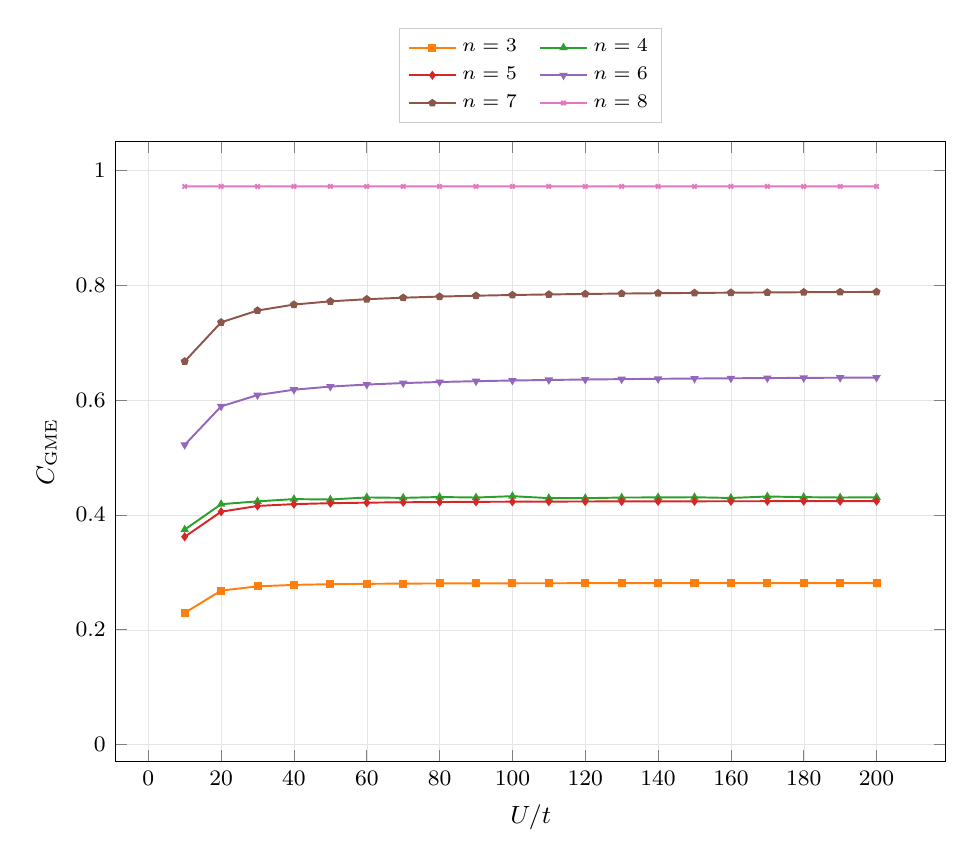
\begin{tikzpicture}
  \begin{axis}[
    width=\columnwidth,
    height=0.78\columnwidth,
    xlabel={$U/t$},
    ylabel={$C_{\mathrm{GME}}$},
    grid=both,
    grid style={line width=.1pt, draw=gray!20},
    tick label style={font=\footnotesize\rmfamily, /pgf/number format/fixed},
    label style={font=\small\rmfamily},
    scaled ticks=false,
    legend style={font=\scriptsize\rmfamily, draw=gray!40, at={(0.5,1.03)}, anchor=south, /tikz/every even column/.append style={column sep=6pt}},
    legend cell align={left},
    legend columns=2,
    ymin=-0.03,
    ymax=1.05,
  ]
    \addplot[color=gmeC1, mark=square*, mark size=1.1pt, line width=0.7pt] coordinates {
        (10,0.229253) (20,0.268065) (30,0.275405) (40,0.277978)
        (50,0.279169) (60,0.279816) (70,0.280207) (80,0.28046)
        (90,0.280634) (100,0.280758) (110,0.28085) (120,0.28092)
        (130,0.280974) (140,0.281017) (150,0.281052) (160,0.281081)
        (170,0.281104) (180,0.281124) (190,0.281141) (200,0.281155)
    };
    \addlegendentry{$n=3$}
    \addplot[color=gmeC2, mark=triangle*, mark size=1.1pt, line width=0.7pt] coordinates {
        (10,0.374228) (20,0.418465) (30,0.423471) (40,0.427345)
        (50,0.426668) (60,0.430259) (70,0.429508) (80,0.430991)
        (90,0.430105) (100,0.432457) (110,0.429075) (120,0.428966)
        (130,0.430075) (140,0.430325) (150,0.430594) (160,0.429335)
        (170,0.431891) (180,0.430794) (190,0.430143) (200,0.430453)
    };
    \addlegendentry{$n=4$}
    \addplot[color=gmeC3, mark=diamond*, mark size=1.1pt, line width=0.7pt] coordinates {
        (10,0.361732) (20,0.40539) (30,0.41545) (40,0.418604)
        (50,0.42023) (60,0.421192) (70,0.421828) (80,0.422274)
        (90,0.422607) (100,0.422853) (110,0.423054) (120,0.423212)
        (130,0.423341) (140,0.423451) (150,0.423545) (160,0.423627)
        (170,0.423695) (180,0.423755) (190,0.423808) (200,0.423856)
    };
    \addlegendentry{$n=5$}
    \addplot[color=gmeC4, mark=triangle*, mark size=1.1pt, mark options={rotate=180}, line width=0.7pt] coordinates {
        (10,0.521815) (20,0.588868) (30,0.608537) (40,0.617848)
        (50,0.623313) (60,0.626885) (70,0.629408) (80,0.631283)
        (90,0.632734) (100,0.633889) (110,0.634831) (120,0.635614)
        (130,0.636275) (140,0.636841) (150,0.637332) (160,0.637759)
        (170,0.638136) (180,0.638472) (190,0.638769) (200,0.639038)
    };
    \addlegendentry{$n=6$}
    \addplot[color=gmeC5, mark=pentagon*, mark size=1.1pt, line width=0.7pt] coordinates {
        (10,0.667188) (20,0.735218) (30,0.755754) (40,0.766131)
        (50,0.771751) (60,0.775461) (70,0.778092) (80,0.780055)
        (90,0.781576) (100,0.782789) (110,0.783778) (120,0.784601)
        (130,0.785296) (140,0.785891) (150,0.786405) (160,0.786855)
        (170,0.787252) (180,0.787604) (190,0.787919) (200,0.788202)
    };
    \addlegendentry{$n=7$}
    \addplot[color=gmeC6, mark=x, mark size=1.1pt, line width=0.7pt] coordinates {
        (10,0.97189) (20,0.971887) (30,0.971886) (40,0.971886)
        (50,0.971886) (60,0.971886) (70,0.971886) (80,0.971886)
        (90,0.971886) (100,0.971886) (110,0.971886) (120,0.971886)
        (130,0.971886) (140,0.971886) (150,0.971886) (160,0.971886)
        (170,0.971886) (180,0.971886) (190,0.971886) (200,0.971886)
    };
    \addlegendentry{$n=8$}
  \end{axis}
\end{tikzpicture}
